\documentclass[10pt, pdf,xcolor=pdftex,dvipsnames,table]{beamer}

\usepackage[brazil]{babel}
\usepackage[utf8]{inputenc}
\usepackage[T1]{fontenc}

\usepackage{pgfpages}
%\usepackage{fancyvrb}
\usepackage{times}
%\usepackage{pgf,pgfarrows,pgfnodes,pgfautomata,pgfheaps}
\usepackage{amsmath,amssymb}
\usepackage{graphicx}
\usepackage{color}
\usepackage{hyperref}
\usepackage{pxfonts,txfonts}
\usepackage{url}
\usefonttheme{structurebold}
\usepackage{hyphenat}
\usepackage{multicol}
\usepackage{fp}
\usepackage{fancyvrb}
\usepackage{xcolor}
%\usepackage{enumitem}

\usepackage{pgfplots}
\usepackage{pgfplotstable}
\usepackage{tikz}
\usetikzlibrary{patterns}

\definecolor{purpleheart}{rgb}{0.41, 0.21, 0.61}

\definecolor{airforceblue}{rgb}{0.36, 0.54, 0.66}

\definecolor{arylideyellow}{rgb}{0.91, 0.84, 0.42}

\definecolor{caribbeangreen}{rgb}{0.0, 0.8, 0.6}

\definecolor{cerulean}{rgb}{0.0, 0.48, 0.65}

\definecolor{terracotta}{rgb}{0.89, 0.45, 0.36}

\definecolor{tangelo}{rgb}{0.98, 0.3, 0.0}

\definecolor{dodgerblue}{rgb}{0.12, 0.56, 1.0}

\definecolor{tractorred}{rgb}{0.99, 0.05, 0.21}

\definecolor{brickred}{rgb}{0.8, 0.25, 0.33}

\definecolor{camouflagegreen}{rgb}{0.47, 0.53, 0.42}

%\usepackage{listings} % para inserir codigo fonte
%\lstset{extendedchars=true,
%breaklines=true,
%frame=tb,
%basicstyle=\footnotesize,
%stringstyle=\ttfamily,
%showstringspaces=false
%}

%\renewcommand{\lstlistingname}{Listagem}

\newcommand{\x}{\textbf{\textcolor{Green}{$\surd$}}}
\newcommand{\xx}{\textbf{\textcolor{Blue}{$\odot$}}}
\newcommand{\xxx}{\textbf{\textcolor{Red}{$\times$}}}

\newcommand{\tf}{\cellcolor{green!65}}
\newcommand{\tp}{\cellcolor{blue!65}}
\newcommand{\tn}{\cellcolor{yellow!65}}


% Comandos para auxiliar na construção de gráficos via latex

\usetheme{Amsterdam}
\setbeamertemplate{navigation symbols}{}

\pgfdeclareimage[height=1.5cm]{logo}{images/lups_oficial.png}
\logo{%
	%\hspace{5cm}
	%
\includegraphics[width=1cm,height=1cm,keepaspectratio]{images/lups_oficial.png}
	\hspace{5cm}
	\pgfuseimage{logo}
}

\setbeameroption{hide notes}

%==================================================================================

%EVENTO
\renewcommand{\evento}{Defesa de Mestrado}

% TITULO DA APRESENTACAO
\title{LTMS - Lups Transactional Memory Scheduler: Um escalonador NUMA-Aware para STM.}

%Autor
\author{\textbf{Michael Alexandre Costa}\\
\and Prof. Dr. André Rauber Du Bois (Orientador) \\
}

%%%%%%%%%%%%%%%%%%%%%%%%%%%%%%%%%%%%%%%%
% Instituição
%%%%%%%%%%%%%%%%%%%%%%%%%%%%%%%%%%%%%%%%

\institute{Mestrado em Computação \\ Centro de Desenvolvimento Tecnológico \\ Universidade Federal de Pelotas \\
\url{macosta@inf.ufpel.edu.br} 
}

\date{\today}

\begin{document}

% % % % % % % % % % % % % % % % % % % % % %
\frame{\titlepage}
\pgfdeclareimage[height=0.7cm]{logo}{images/lups_timbre.png}
\logo{%
	\pgfuseimage{logo}
}


% % % % % % % % % % % % % % % % % % % % % %
\frame{\tableofcontents}

%%%%%%%%%%%%%%%%%%%%%%%%%%%%%%%%%%%%%%%%%%%%%
% Conteúdo da Apresentação
%%%%%%%%%%%%%%%%%%%%%%%%%%%%%%%%%%%%%%%%%%%%%

\section{Introdução}

\begin{frame} \frametitle{Introdução}
    \begin{block}{Motivação}
        \begin{itemize}
        	\item Programação Paralela;
        	\item Memórias Transacionais;
        	\item Escalonadores de Transações; e
        	\item Arquiteturas NUMA.
        \end{itemize}
    \end{block}
\end{frame}

\begin{frame} \frametitle{Introdução}
    \begin{block}{Objetivos}
        \begin{itemize}
        	\item Projetar um escalonador de STM modular que considera a arquitetura utilizada, intitulado LTMS;
        	\item Prototipar o escalonador LTMS, utilizando a biblioteca de STM TinySTM; e
			\item Análisar de desempenho do LTMS comparado a TinySTM utilizando o conjunto de benchmarks STAMP.
        \end{itemize}
    \end{block}
\end{frame}

\section{Memórias Transacionais}

\begin{frame} \frametitle{Memórias Transacionais}
    \begin{block}{Características}
        \begin{itemize}
        	\item Fornece abstração de código;
        	\item Reuso de código; e
        	\item Ausência de deadlocks.
        \end{itemize}
    \end{block}
    
    \begin{block}{Transações}
        \begin{itemize}
        	\item Atomicidade;
        	\item Consistência; e
        	\item Isolamento.
        \end{itemize}
    \end{block}
\end{frame}

% \begin{frame} \frametitle{Memórias Transacionais}
%     \begin{block}{Controle das transações}
%         \begin{itemize}
%     		\item Versionamento de Dados:
%     		\begin{itemize}
%     			\item Adiantado / Tardio.
%     		\end{itemize}
%     		\item Detecção de Conflitos:
%     		\begin{itemize}
%     			\item Adiantado / Tardio.
%     		\end{itemize}
%     		\item Gerenciamento de Contenção:
%         		\begin{itemize}
%         		    \item Suicide, Delay, Backoff ou Modular.
%         		\end{itemize}
%         \end{itemize}
%     \end{block}
% \end{frame}

% \begin{frame} \frametitle{Memórias Transacionais}
% \begin{block}{Versionamento Adiantado}
% \begin{itemize}
% 	\item Escreve os dados especulativos direto na memória; e
% 	\item Em caso de um cancelamento, a operação deve ser desfeita.
% \end{itemize}
% % \begin{figure}[!h]
% % 	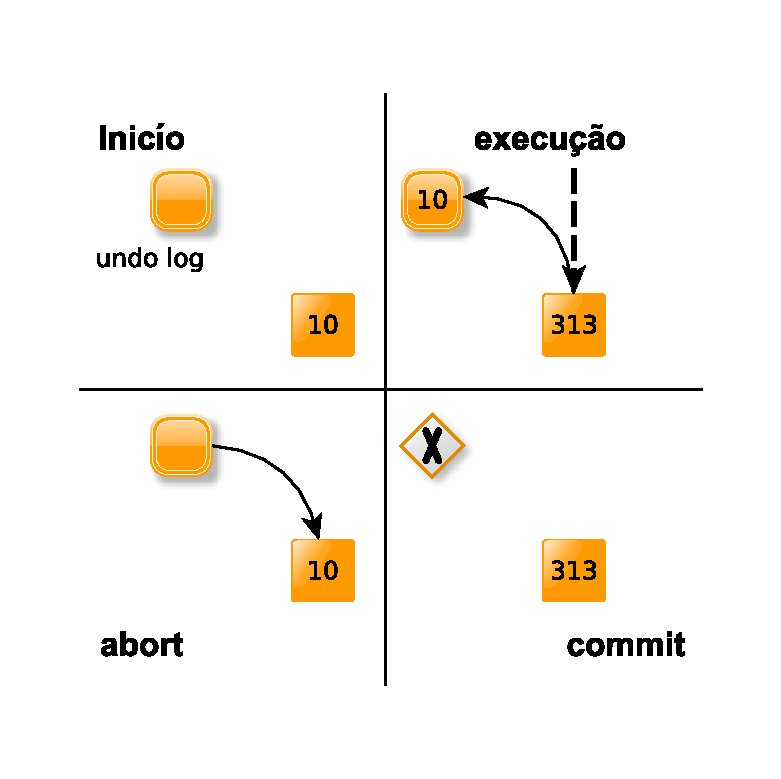
\includegraphics[scale=0.3]{images/versionamento_adiantado}
% % 	\caption{Versionamento Adiantado}
% % 	\label{fig:abusy}
% % \end{figure}
% \end{block}
% \begin{block}{Versionamento Tardio}
% \begin{itemize}
% 	\item Escreve os dados especulativos em um \textit{buffer} local; e
% 	\item Em caso de efetivação, os dados devem ser copiados para a memória.
% \end{itemize}
% % \begin{figure}[!h]
% % 	\centering
% % 	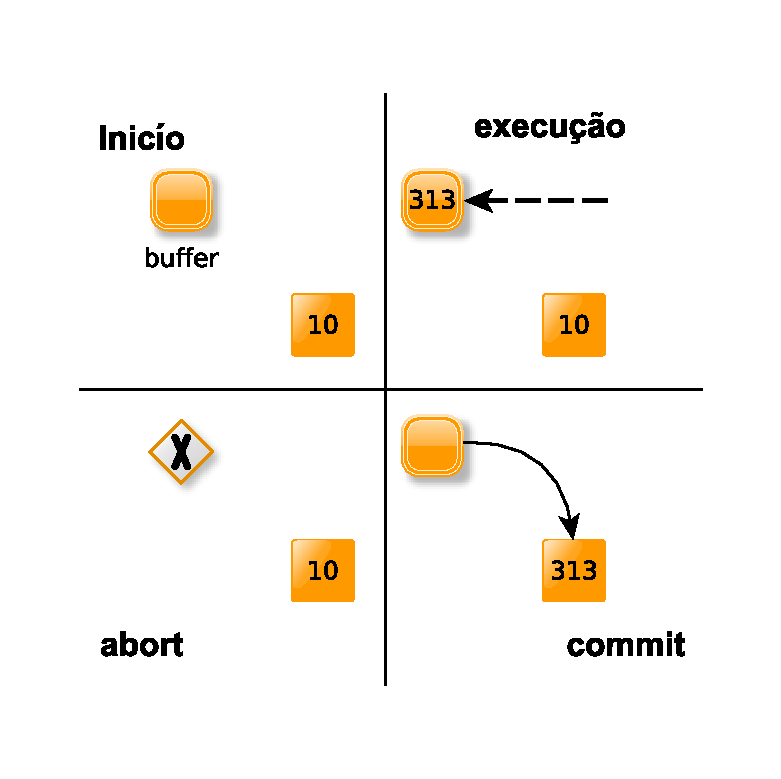
\includegraphics[scale=0.3]{images/versionamento_tardio}
% % 	\caption{Versionamento Tardio}
% % 	\label{fig:abusy}
% % \end{figure}
% % \begin{figure}[!h]
% % 	\centering
% % 	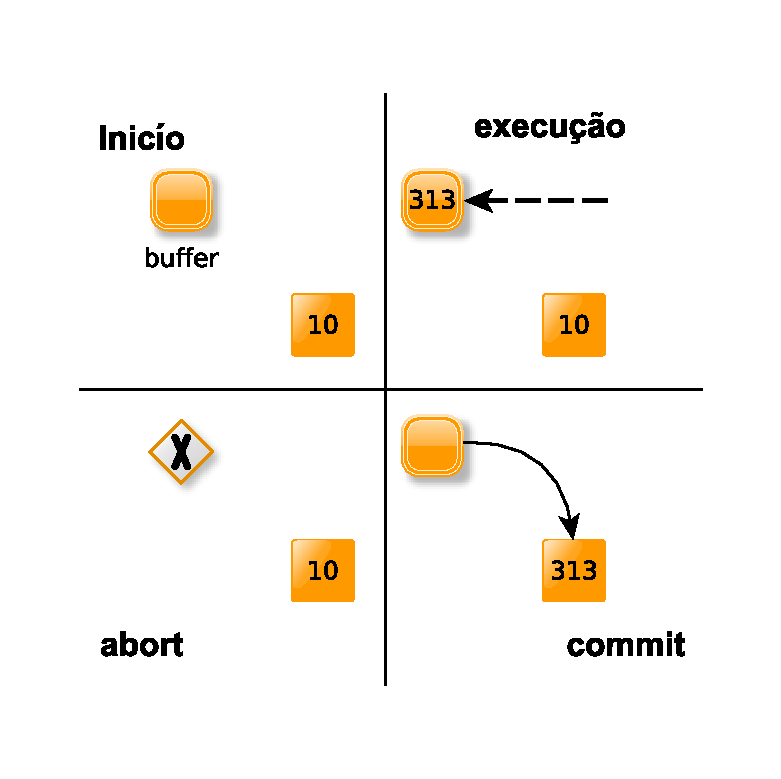
\includegraphics[scale=0.3]{images/versionamento_tardio}
% % 	\caption{Versionamento Tardio}
% % 	\label{fig:abusy}
% % \end{figure}
% \end{block}
% \end{frame}

% \begin{frame} \frametitle{Memórias Transacionais}
% \begin{block}{Detecção de Conflitos Adiantada}
% \begin{itemize}
% 	\item Detecta conflito no momento do acesso a memória.
% \end{itemize}
% % \begin{figure}[!h]
% % 	\centering	
% % 	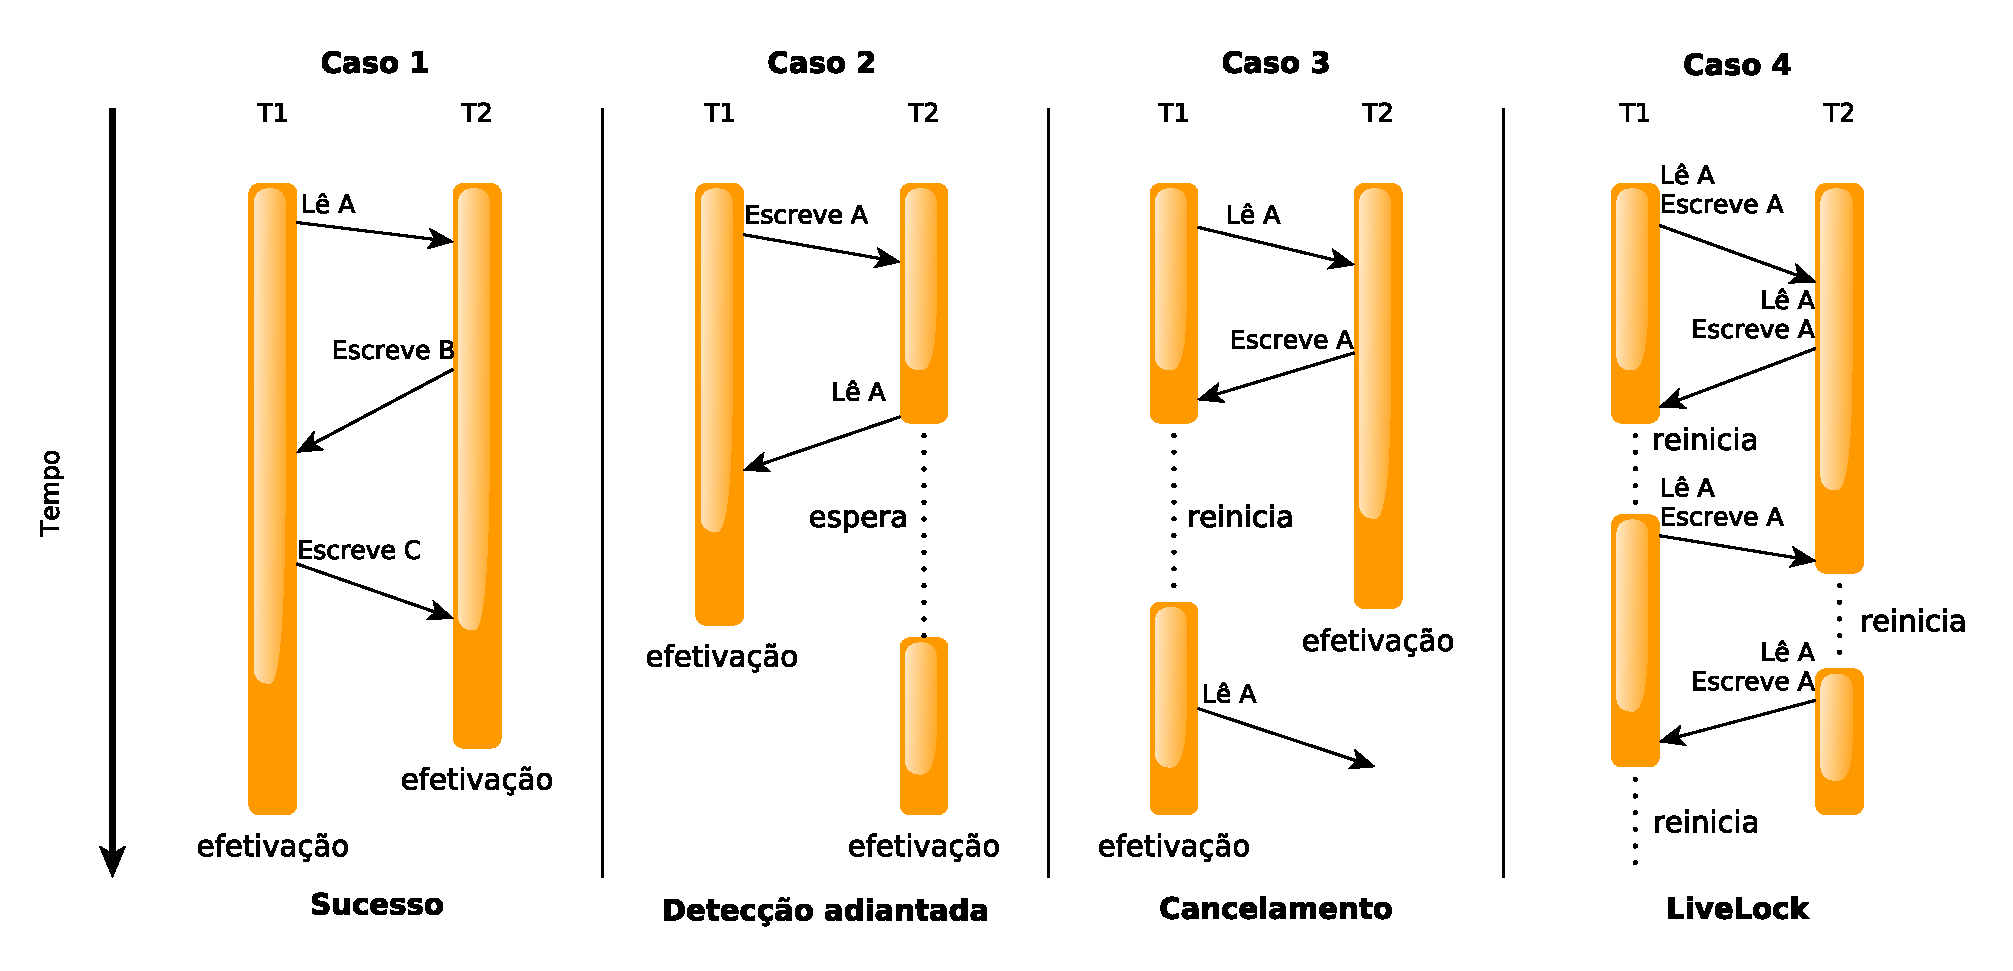
\includegraphics[scale=0.3]{images/deteccao_adiantada}
% % 	\caption{Detecção Adiantada}
% % 	\label{fig:abusy}
% % \end{figure}
% \end{block}
% \begin{block}{Detecção de Conflitos Tardia}
% \begin{itemize}
% 	\item Detecta conflito somente na validação.
% \end{itemize}
% % \begin{figure}[!h]
% % 	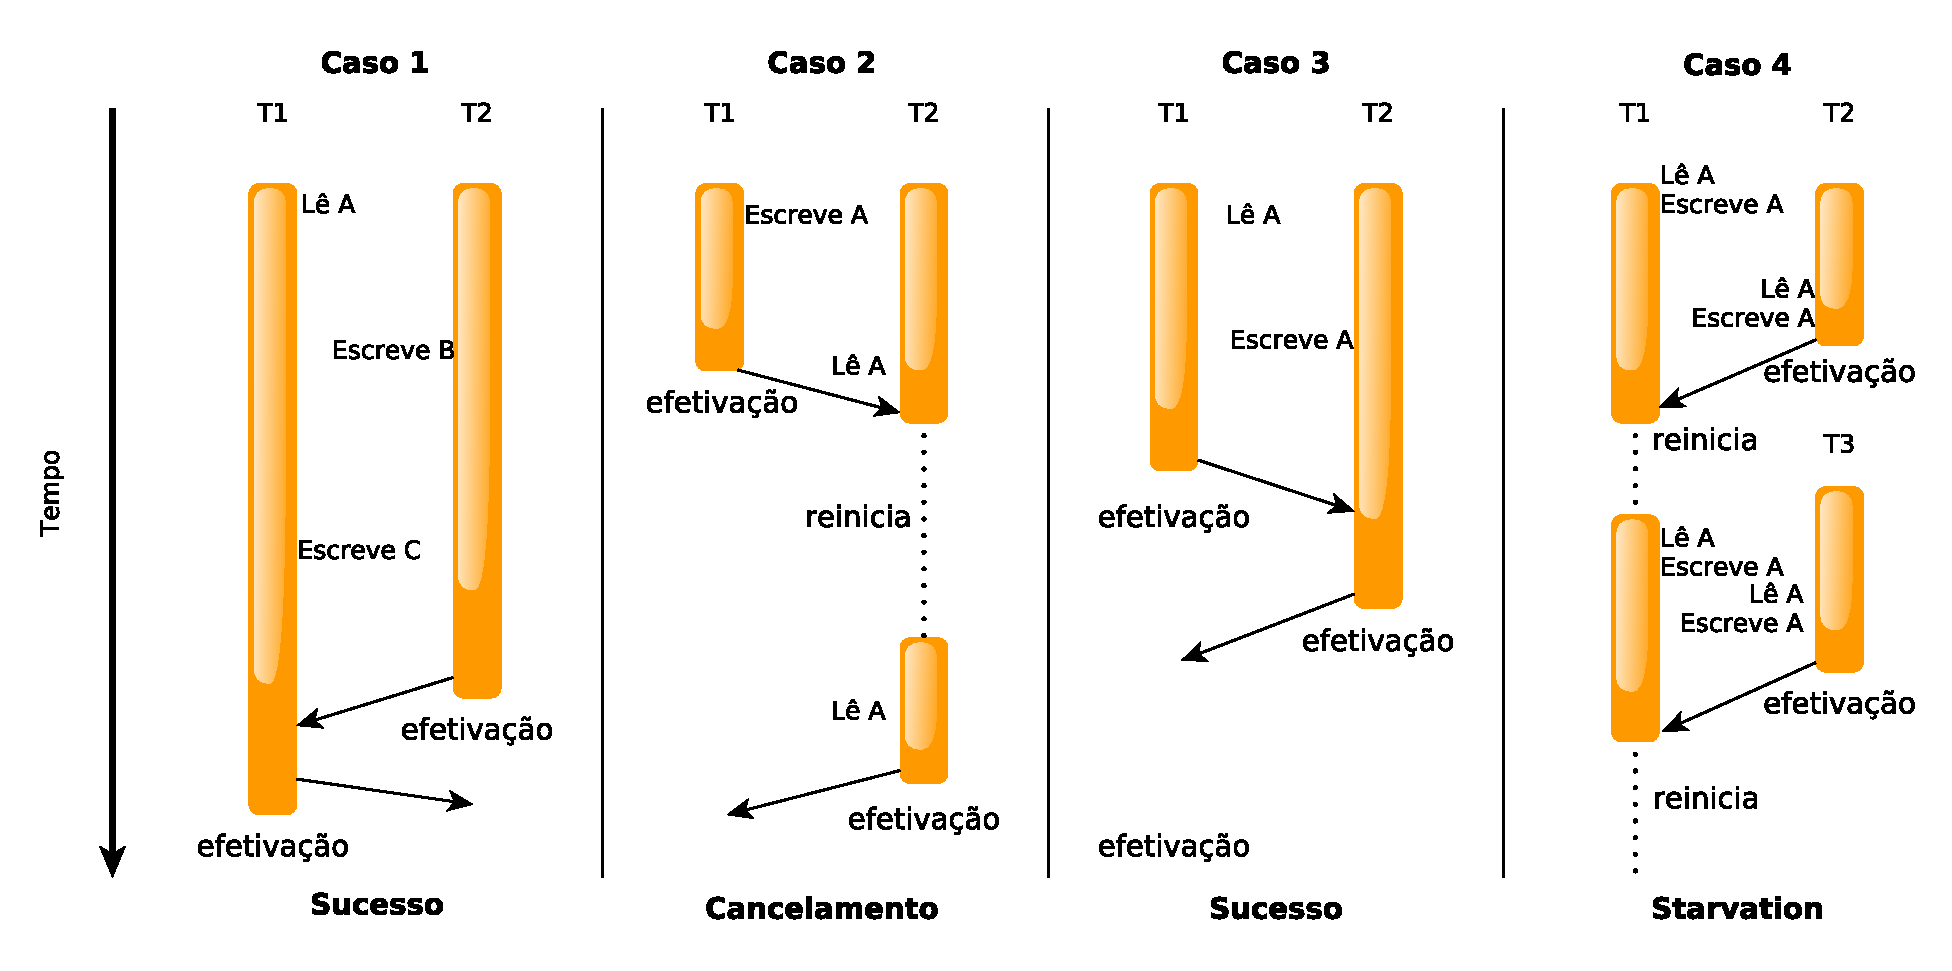
\includegraphics[scale=0.3]{images/deteccao_tardio}
% % 	\caption{Detecção Tardia}
% % 	\label{fig:abusy}
% % \end{figure}
% \end{block}
% \end{frame}

% \begin{frame} \frametitle{Memórias Transacionais}
%     \begin{block}{Gerenciador de Contenção}
%         \begin{itemize}
%         	\item Possui ação reativa;
%         	\item Suicide, Delay, Backoff ou Modular.
%         % 	\begin{itemize}
%         % 	    \item Suicide, Delay, Aggressive, e Timestamp.
%         %     \end{itemize}
%         \end{itemize}
%     \end{block}
%     \begin{block}{Gerenciador de Contenção}
%         \begin{itemize}
%             \item Modular:
%             \begin{itemize}
%     	        \item Suicide, Delay, Aggressive, e Timestamp.
%             \end{itemize}
%         \end{itemize}
%     \end{block}
%     % \begin{alertblock}{Problemas}
%     %     \begin{itemize}
%     %     	\item Somente reinicia a transação conflitante;
%     %     	\item Não evita que conflitos futuros aconteçam; e
%     %     	\item Em ambientes de alta contenção, tende a perder desempenho.
%     %     \end{itemize}
%     % \end{alertblock}
% \end{frame}

\begin{frame} \frametitle{Memórias Transacionais}
    % \begin{block}{Gerenciador de Contenção}
    %     \begin{itemize}
    %     	\item Possui ação reativa;
    %     	\item Suicide, Delay, Backoff ou Modular.
    %     % 	\begin{itemize}
    %     % 	    \item Suicide, Delay, Aggressive, e Timestamp.
    %     %     \end{itemize}
    %     \end{itemize}
    % \end{block}
    % \begin{block}{Modular}
    %     \begin{itemize}
    % 	    \item Suicide, Delay, Aggressive, e Timestamp.
    %     \end{itemize}
    % \end{block}
    \begin{alertblock}{Problemas}
        \begin{itemize}
        	\item Somente reinicia a transação conflitante;
        	\item Não evita que conflitos futuros aconteçam; e
        	\item Em ambientes de alta contenção, tende a perder desempenho.
        \end{itemize}
    \end{alertblock}
\end{frame}

\section{Escalonadores}
\begin{frame} \frametitle{Escalonadores}
\begin{block}{Escalonadores de Transações}
\begin{itemize}
	\item Buscam reduzir os números de conflitos;
	\item Utilizam diferentes Heurísticas de escalonamento; e
	\item Serializa as transações conflitantes.
\end{itemize}
\end{block}
\end{frame}

\begin{frame} \frametitle{Escalonadores}
\begin{block}{Classificação das técnicas}
\begin{itemize}
	\item Baseado em Heurística:
	\begin{itemize}
	    \item Feedback;
	    \item Predição;
	    \item Reativo; e
	    \item Heurística Mista.
	\end{itemize}
	\item Baseado em Modelo:
	\begin{itemize}
	    \item Aprendizado de Máquina;
	    \item Modelo Analítico; e
	    \item Modelo Misto.
	\end{itemize}
\end{itemize}
\end{block}
\end{frame}


\begin{frame} \frametitle{Escalonadores}
\begin{block}{Trabalhos Relacionados}
\begin{table}[]
\footnotesize
\centering
\caption{Algoritmos e técnicas de escalonamento}
\label{tab:compare}
\begin{tabular}{l|l}
\hline
Escalonador & Técnica \\ \hline
ATS & Feedback \\
Probe & Feedback \\
F2C2 & Feedback \\
Shrink & Predição \\
SCA & Predição \\
CAR-STM & Reativo \\
RelSTM & Reativo \\
LUTS & Heurística Mista \\
ProVIT & Heurística Mista \\
SAC-STM & Aprendizado de Máquina \\
CSR-STM & Modelo Analítico \\
MCATS & Modelo Analítico \\
AML & Modelo Misto \\
\hline
\end{tabular}
\end{table}
\end{block}
\end{frame}

\begin{frame} \frametitle{Escalonadores}
\begin{block}{Trabalhos Relacionados}
\begin{table}[]
\footnotesize
\centering
\caption{Algoritmos que estamos trabalhando}
\label{tab:compare}
\begin{tabular}{l|l}
\hline
Escalonador & Técnica \\ \hline
Probe & Feedback \\
F2C2 & Feedback \\
Shrink & Predição \\
MCATS & Modelo Analítico \\
\hline
\end{tabular}
\end{table}
\end{block}
\end{frame}

% \begin{frame} \frametitle{Escalonadores}
% \begin{block}{Shrink}
% \begin{itemize}
%     \item Bloom filter: Utiliza os dados de leitura e escrita por thread:
%     \begin{itemize}
%         \item Conjunto de leitura: Localidade temporal; e
%         \item Conjunto de escrita: Ocorre apenas nos aborts.
%     \end{itemize}
%     \item Serialization affinity: Serializa uma thread de acordo com a contenção do sistema; e
%     \item O escalonador é ativado com base no número de contenção existente.
% \end{itemize}
% \end{block}
% \end{frame}

\section{Arquiteturas}
\begin{frame} \frametitle{Arquiteturas}
\begin{block}{UMA}
\begin{itemize}
	\item Uniform Memory access;
	\item Possui um único barramento de acesso à memória; e
	\item Único custo de acesso à memória.
\end{itemize}
\end{block}
\begin{block}{NUMA}
\begin{itemize}
	\item Non-uniform Memory access;
	\item Possui mais de um barramento de acesso à memória; e
	\item O custo de acesso à memória é diferente conforme o núcleo utilizado.
\end{itemize}
\end{block}
\end{frame}

\section{Objetivos}
\begin{frame} \frametitle{Objetivos}
\begin{block}{Objetivos}
\begin{itemize}
	\item Estudar o comportamento dos escalonadores na arquitetura NUMA;
	\item Inserir as novas regras de escalonamento para arquitetura NUMA.
\end{itemize}
\end{block}
\end{frame}

\begin{frame} \frametitle{Metodologia}
    \begin{block}{Ferramentas utilizadas}
        \begin{itemize}
        	\item Shrink;
        	\item TinySTM;
        	\item Hwloc; e
        	\item STAMP.
        \end{itemize}
    \end{block}
\end{frame}

\begin{frame} \frametitle{Metodologia}
\begin{block}{O que foi feito}
    \begin{itemize}
        \item Foi implementado um escalonador com filas de threads para cada núcleo;
        \item Foi feito um escalonador que migra threads;
    	\item Foram estudados os algoritmos de escalonamentos atuais; e
    	\item Foi desenvolvido um novo fluxo de execução para o Shrink.
    \end{itemize}
\end{block}
\end{frame}

\begin{frame} \frametitle{Metodologia}
\begin{block}{O que será feito}
\begin{itemize}
	\item Modificar a implementação de threads do Shrink para utilizar filas;
	\item Coletar informações da latência de acordo com o Bloom Filter; e
	\item Adicionar a migração de threads ao Shrink.
\end{itemize}
\end{block}
\end{frame}

\begin{frame} \frametitle{Metodologia}
\begin{block}{Modificações e nomenclatura}
\begin{itemize}
	\item Cada núcleo possuirá uma fila de threads que chamamos de Qn;
	\item O escalonador possuirá uma fila de threads inicial chamada de Pt; e
	\item Uma Thread (Tn) pode ter n transações que chamamos de Tr.
\end{itemize}
\end{block}
\end{frame}

\begin{frame} \frametitle{Metodologia}
    \begin{figure}[!h]
	    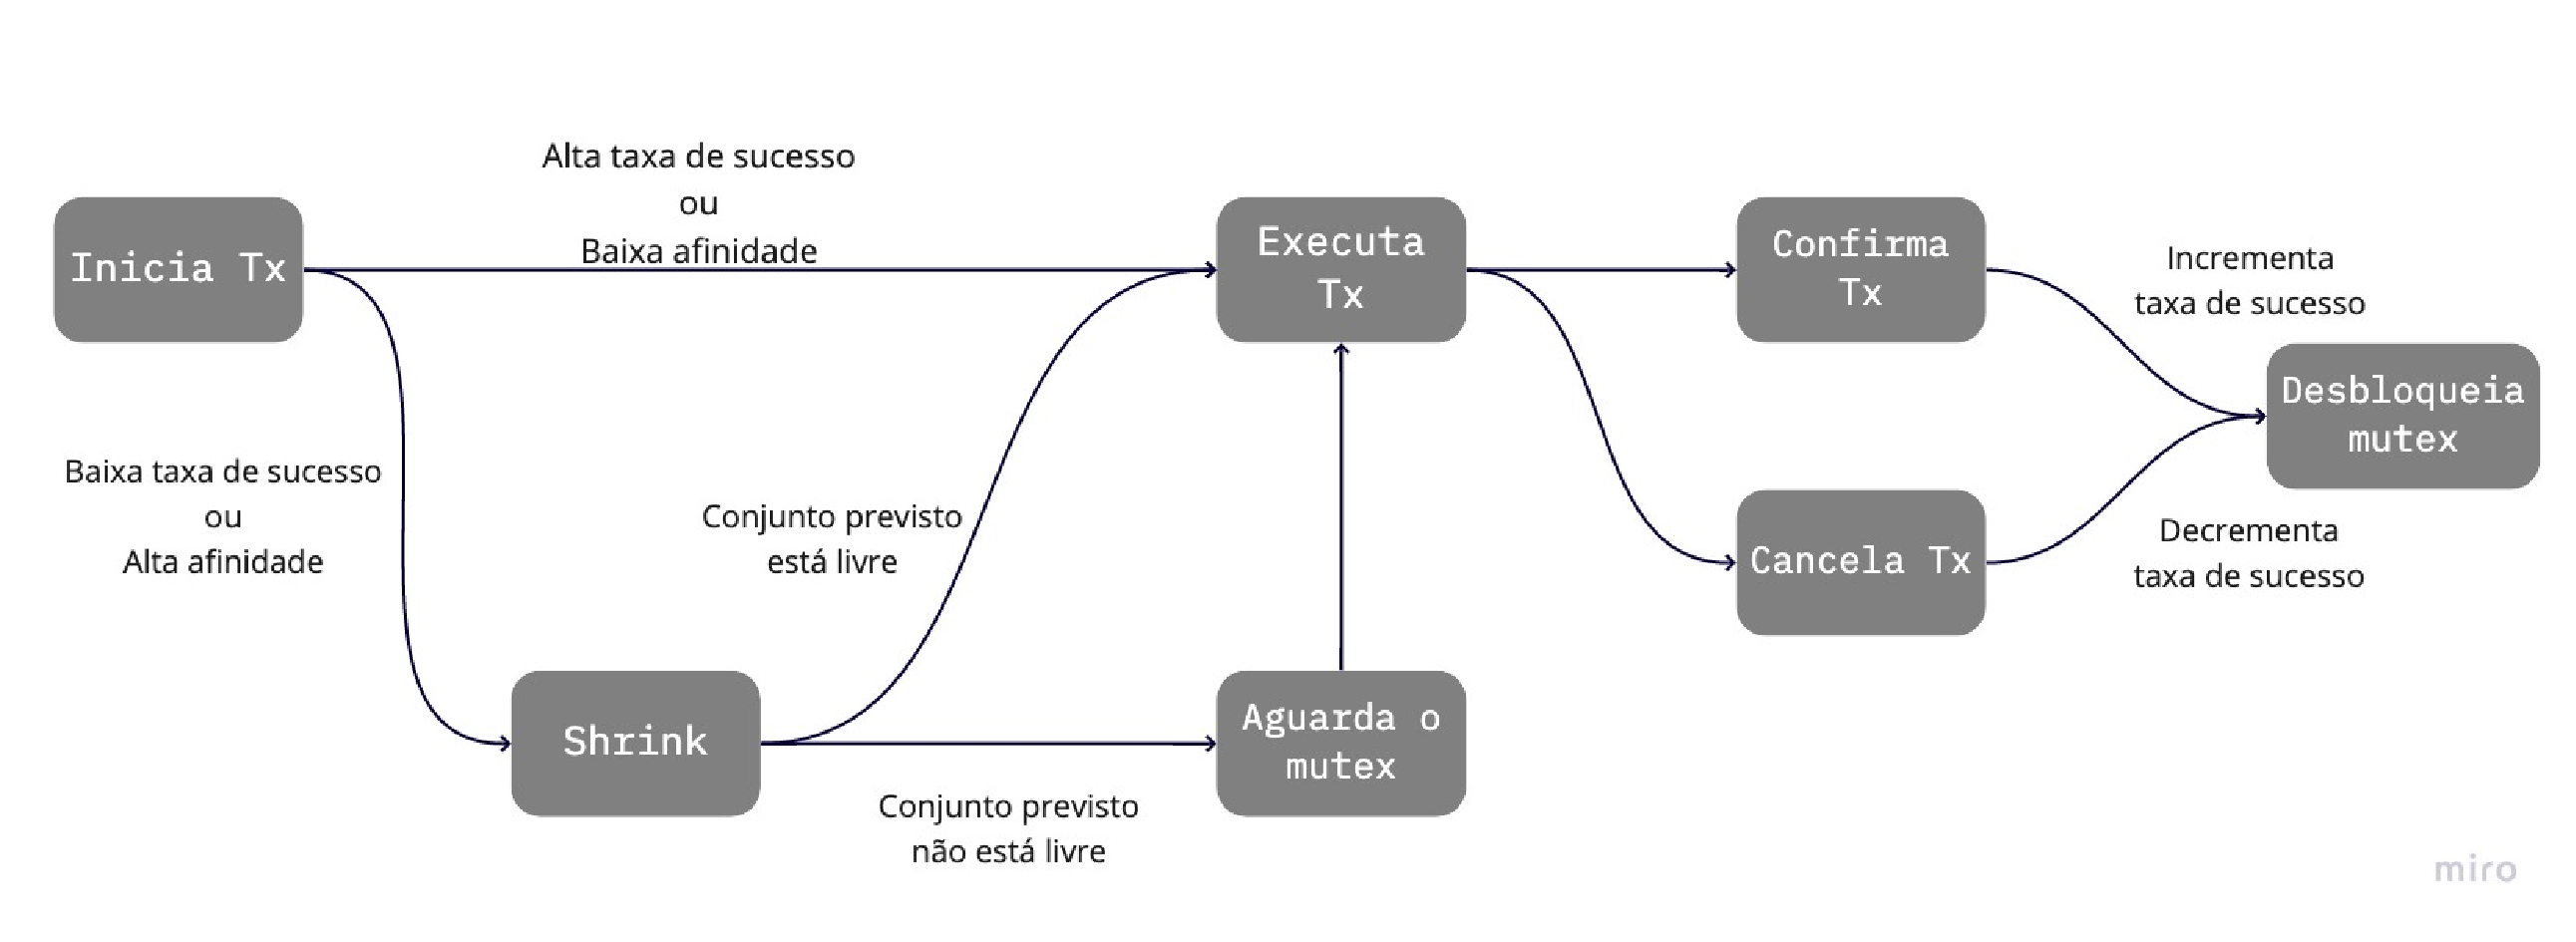
\includegraphics[scale=0.25]{images/ShrinkFlow}
	    \caption{Shrink}
	    \label{fig:abusy}
    \end{figure}
\end{frame}

\begin{frame} \frametitle{Metodologia}
    \begin{figure}[!h]
	    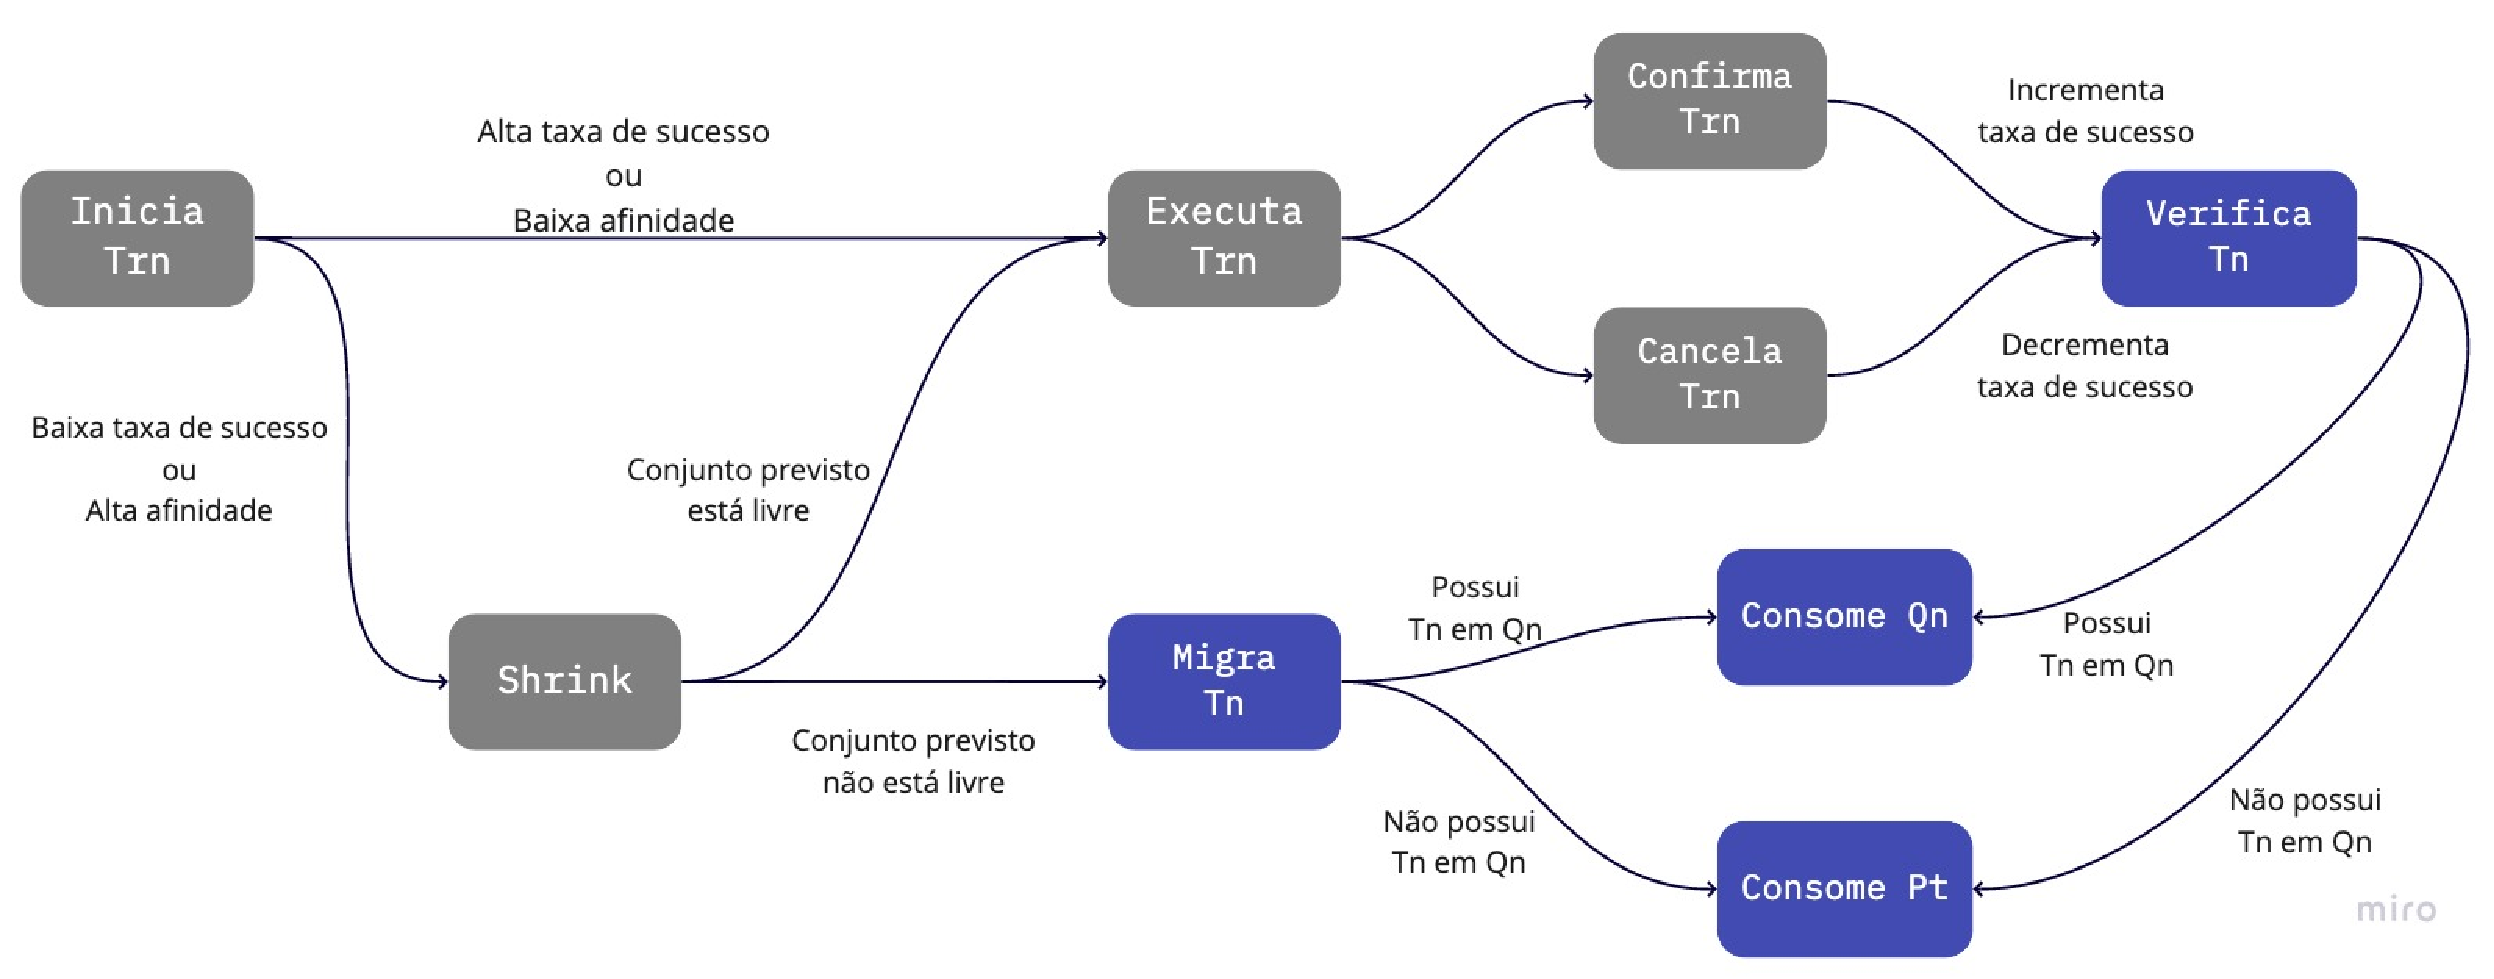
\includegraphics[scale=0.25]{images/LScheduleFlow}
	    \caption{Modificações}
	    \label{fig:abusy}
    \end{figure}
\end{frame}

\section{Próximas Atividades}
\begin{frame} \frametitle{Próximas Atividades}
\begin{block}{Atividades a serem realizadas}
\begin{itemize}
	\item Modificar o escalonador Shrink;
	\item Executar os testes;
	\item Analisar resultados; e
	\item Escrever a Dissertação.
\end{itemize}
\end{block}
\end{frame}

\section{Cronograma de Atividades}

\begin{frame} \frametitle{Cronograma}
\begin{enumerate}
	\item Modificações no Shrink coletando informações sobre a arquitetura;
	\item Modificações no método de escalonamento do Shrink;
	\item Validação do novo método de escalonamento;
	\item Execução de testes em arquitetura NUMA e UMA;
	\item Coleta de resultados obtidos por meio dos testes;
	\item Escrita da dissertação; e
	\item Entrega e apresentação da dissertação.
\end{enumerate}
\end{frame}

\begin{frame} \frametitle{Cronograma}
\begin{table}[!h]
\centering
\caption{Cronograma de atividades mensal para o restante do mestrado}
\label{tab:cro2}
\scalebox{0.75}{
	\begin{tabular}{c|c|c|c|c|c|c|c} \hline
		Ano & \multicolumn{5}{|c|}{2020} & \multicolumn{2}{|c}{2021} \\ \hline
		Mês & Ago & Set & Out & Nov & Dez & Jan & Fev \\ \hline
		1   & \tn & \tn & \tn & &   &   &   \\ \hline
		2   &   & \tn & \tn & \tn & &   & \\ \hline
		3   &   &   &   & \tn & \tn & &   \\ \hline
		4   &   &   &   &   & \tn & \tn & \\ \hline
		5   &   &   &   &   & & \tn &  \tn \\ \hline
		6   &   & \tn & \tn & \tn & \tn & \tn & \tn \\ \hline
		7   &   &   & &   & & & \tn \\ \hline	
\end{tabular}
}
\end{table}
\end{frame}
\maketitle
\end{document}

